\documentclass[reqno]{amsart}

\usepackage{amsfonts,latexsym,amsthm,amssymb,amsmath,amscd,euscript,bm}
\usepackage[sc]{mathpazo}
\usepackage[margin = 2.6cm]{geometry}
\usepackage{enumitem}
\usepackage{hyperref}
% sets numbering of enumerate to a, b, c, ...
\renewcommand{\theenumi}{\alph{enumi}}

% Theorems, propositions, etc.
\newtheorem{theorem}{Theorem}
\newtheorem{proposition}[theorem]{Proposition}
\newtheorem{lemma}[theorem]{Lemma}
\newtheorem{corollary}[theorem]{Corollary}

\theoremstyle{definition}
\newtheorem{definition}[theorem]{Definition}
\newtheorem*{claim}{Claim}

\theoremstyle{remark}
\newtheorem*{remark}{Remark}
\newtheorem*{notation}{Notation}

\usepackage{tikz-cd}

\usepackage{graphicx}


% Math blackboard font
\newcommand{\nc}{\newcommand}
\nc{\on}[1]{\operatorname{#1}}

\nc{\R}{\mathbb R}
\nc{\C}{\mathbb C}
\nc{\Q}{\mathbb Q}
\nc{\Z}{\mathbb Z}
\nc{\N}{\mathbb N}
\nc{\HH}{\mathbb H}
\nc{\DD}{\mathbb D}
\nc{\TT}{\mathbb T}
\nc{\EE}{\mathbb E}
\nc{\PP}{\mathbb P}

\nc{\cT}{\mathcal T}
\nc{\cA}{\mathcal A}
\nc{\cM}{\mathcal M}
\nc{\cR}{\mathcal R}
\nc{\cB}{\mathcal B}
\nc{\cG}{\mathcal G}
\nc{\cD}{\mathcal D}
\nc{\cS}{\mathcal S}
\nc{\cF}{\mathcal F}
\nc{\cL}{\mathcal L}
\nc{\cE}{\mathcal E}

\nc{\diam}{\operatorname{diam}}
\nc{\supp}{\operatorname{supp}}
\nc{\loc}{\text{loc}}

% Why the f*** would you ever use \epsilon
\renewcommand{\epsilon}{\varepsilon}
\renewcommand{\emph}{\textsc}

\renewcommand{\Re}{\operatorname{Re}}
\renewcommand{\Im}{\operatorname{Im}}
%inverse Fourier transform widecheck
\DeclareFontFamily{U}{mathx}{\hyphenchar\font45}
\DeclareFontShape{U}{mathx}{m}{n}{
      <5> <6> <7> <8> <9> <10>
      <10.95> <12> <14.4> <17.28> <20.74> <24.88>
      mathx10
      }{}
\DeclareSymbolFont{mathx}{U}{mathx}{m}{n}
\DeclareFontSubstitution{U}{mathx}{m}{n}
\DeclareMathAccent{\widecheck}{0}{mathx}{"71}

\let\vec\mathbf

% Title: change problem set number as needed
\title
{
	\emph{Interpolation of Lebesgue and Lorentz spaces}
} 

\author{Jason Zhao}
\date{\today}

\begin{document}
\maketitle

\begin{abstract}
	Given an operator $T$ bounded between two pairs of function spaces, the problem of \textit{interpolation} asks: what can we say about the boundedness of $T$ between function spaces \textit{interpolated} between our original spaces? We set the stage by defining the Lorentz function space $L^{p, q} (X)$ and present both the complex and real methods for interpolating bounds on linear and sub-linear operators. These notes are inspired by \cite{Tao2006}; for a textbook treatment, see \cite{Grafakos2014}. 
\end{abstract}

\tableofcontents

\section{Lebesgue spaces}

Let $(X, \mu)$ be a measure space and $1\leq p \leq \infty$, the \emph{$L^p$ space}, denoted $L^p (X)$, is the space of measurable functions $f: X \to \C$ such that the norm
	\begin{alignat*}{2}
		||f||_{L^p} 
			&:= \left( \int_X |f|^p d \mu \right)^{1/p}, 
			&&\qquad \text{when $p \neq \infty$}, \\
		||	f||_{L^\infty}
			&:= \operatorname{ess} \sup_{x \in X} |f(x)|,
			&&\qquad \text{when $p = \infty$,}
	\end{alignat*}
is finite. The quantity above forms a monotone norm, that is, for $f, g \in L^p (X)$ and $\alpha \in \C$, it satisfies the following:
\begin{enumerate}
	\item Monotonicity, if $|f| \leq |g|$, then 
		\[ ||f||_{L^p} \leq ||g||_{L^p}. \]
	\item Positive definiteness, 
		\[||f||_{L^p} \geq 0 \]
	with equality only if $f \equiv 0$. 	
	\item Absolute homogeneity, 
		\[ ||\alpha f||_{L^p} = |\alpha| \, ||f||_{L^p}. \]
	\item The triangle inequality, 
		\[ ||f + g||_{L^p} \leq ||f||_{L^p} + ||g||_{L^p}. \]
\end{enumerate}



\subsection{Complex interpolation}

Let $T$ be an operator mapping a subspace of measurable functions $Y \to \C$ to measurable functions $Y \to \C$, we say it is \emph{linear} if it satisfies
	\[ T(\alpha f + g) = \alpha Tf + Tg \]
for all $\alpha \in \C$ and $f, g : X \to \C$ in the domain of $T$. For $1 \leq p, q \leq \infty$, a linear operator is \emph{strong-type} $(p, q)$ if it is bounded $T: L^p (X) \to L^q(Y)$, i.e. it satisfies the strong-type $(p, q)$ inequality
	\[ ||Tf||_{L^q} \lesssim ||f||_{L^p}, \qquad \text{uniformly in $f \in L^p(X)$.} \]
\begin{proposition}
	Let $T : L^p (X) \to L^q (Y)$ be a linear operator. Then the following are equivalent:
	\begin{enumerate}
		\item $T$ is strong-type $(p, q)$.
		\item $T$ is Lipschitz continuous.
		\item $T$ is continuous at the origin. 
	\end{enumerate}
\end{proposition}
	
\begin{proof}
	From linearity we see that (a) $\implies$ (b) and (b) $\implies$ (c) is trivial, so to close the chain of implications we show (c) $\implies$ (a). Let $\epsilon > 0$, then there exists $\delta > 0$ such that 
		\[ ||Tf||_{L^q} < \epsilon, \qquad \text{whenever } ||f||_{L^p} \leq \delta. \]
	For any $f \in L^p (X)$, we use homogeneity and apply the inequality above to the normalised function $\delta f/||f||_{L^p}$ to obtain the strong-type $(p, q)$ inequality, 
		\[ ||Tf||_{L^q} = \frac{||f||_{L^p}}{\delta} \Big|\Big|T \Big(\delta \frac{f}{||f||_{L^p}}\Big) \Big|\Big|_{L^q} \leq \frac{\epsilon}{\delta} ||f||_{L^p}, \]
	completing the proof. 	
\end{proof}

\begin{remark}
	To avoid any philosophical malaise on whether an operator is well-defined on all $L^p$-functions, it is convenient to consider a linear operator acting on a sufficiently regular sub-class, namely test functions $C^\infty_c (\R^d)$ or Schwartz functions $\cS (\R^d)$. Upon proving a strong-type $(p, q)$ estimate for $p \neq \infty$ for such functions, we can extend the result by density and Lipschitz continuity to all $L^p$-functions. 
\end{remark}

Let $1 \leq p_0, p_1 \leq \infty$ and $0 \leq \theta \leq 1$, define $1 \leq p_\theta \leq \infty$ by 
	\[ \frac{1}{p_\theta} = \frac{1 - \theta}{p_0} + \frac{\theta}{p_1}. \]
The space $L^{p_\theta} (X)$ is known as an \textit{interpolation space} between $L^{p_0} (X)$ and $L^{p_1} (X)$. More precisely, $L^{p_\theta} (X)$ ``lives between'' $L^{p_0} (X)$ and $L^{p_1} (X)$ in the sense that 
	\[ L^{p_0} (X) \cap L^{p_1} (X) \subseteq L^{p_\theta} (X) \subseteq L^{p_0} (X) + L^{p_1} (X).\]
The first inclusion follows from Holder's inequality, writing $f = f^{1 - \theta} f^\theta$, 
		\[ ||f||_{L^{p_\theta}} \leq ||f||_{L^{p_0}}^{1 - \theta} ||f||_{L^{p_1}}^\theta.\]
	The second inclusion follows from decomposing $f = f \mathbb 1_{|f| > 1} + f \mathbb 1_{|f| \leq 1}$, monotonicity of $|x| \mapsto |x|^p$, and noting that $p_0 < p_\theta < p_1$, 
		\[ ||f \mathbb 1_{|f| > 1}||_{L^{p_0}} \leq || f||_{L^{p_\theta}} , \qquad  ||f \mathbb 1_{|f| \leq 1}||_{L^{p_1}} \leq || f||_{L^{p_\theta}}. \]	
Given $1 \leq p_0, p_1, q_0, q_1 \leq \infty$ and a linear operator $T: (L^{p_0} + L^{p_1}) (X) \to (L^{q_0} + L^{q_1}) (Y)$ of strong-type $(p_0, q_0)$ and $(p_1, q_1)$, we see that $T$ forms a map between the interpolation spaces. \textit{Interpolation} is the problem of establishing the strong-type $(p_\theta, q_\theta)$ inequality. 

\begin{figure}[h]
	\begin{center}
		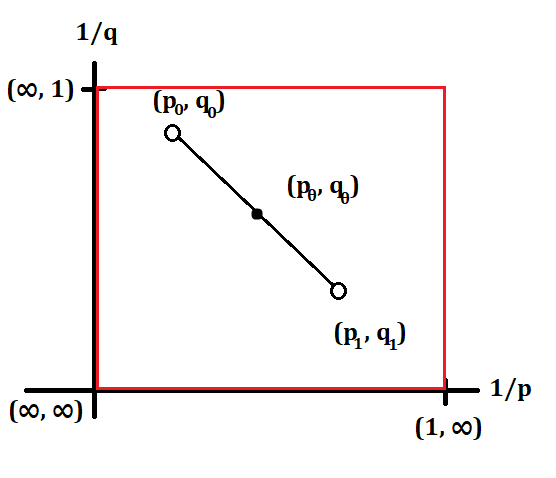
\includegraphics[scale = 0.6]{realinter}
		\caption{The \textit{interpolation diagram}; given bounds for exponents $(p_0, q_0)$ and $(p_1, q_1)$, interpolation furnishes bounds for exponents $(p_\theta, q_\theta)$ on the intermediate line.}
	\end{center}
\end{figure}


\begin{theorem}[Riesz-Thorin interpolation]
	Let $1 \leq p_0, p_1, q_0, q_1 \leq \infty$ and $0 < \theta < 1$, and suppose $(X, \mu)$ and $(Y, \nu)$ are measure spaces, the latter $\sigma$-finite when $q_0 = q_1 = \infty$. If $T: (L^{p_0} + L^{p_1})(X) \to (L^{q_0} + L^{q_1}) (Y)$ is a linear operator of strong-type $(p_0, q_0)$ and $(p_1, q_1)$, i.e.
		\begin{align*}
			||Tf||_{L^{q_0}} 
				&\leq M_0 ||f||_{L^{p_0}}, \qquad \text{uniformly in $f \in L^{p_0} (X)$} \\
			||Tf||_{L^{q_1} (Y)} 
				&\leq M_1 ||f||_{L^{p_1}}, \qquad \text{uniformly in $f \in L^{p_1} (X)$}
		\end{align*}	
	for some $0 < M_0, M_1 < \infty$. Then $T$ satisfies the strong-type $(p_\theta, q_\theta)$ inequality
		\[ ||Tf||_{L^{q_\theta}} \leq M_0^{1 - \theta} M_1^\theta ||f||_{L^{p_\theta}}. \]
\end{theorem}

\begin{proof}
	If $p_0 = p_1 = p_\theta$, the result follows from the log convexity of the $L^p$-norm. That is, by Holder's inequality, 
		\[ || g||_{L^{q_\theta}}^{q_\theta} = \int_Y |g|^{(1 - \theta)q_\theta} |g|^{\theta q_\theta} \, d\nu \leq |||g|^{(1 - \theta)q_\theta} ||_{L^{\frac{q_0}{(1 - \theta)q_\theta}}} |||g|^{\theta q_\theta} ||_{L^\frac{q_1}{\theta q_\theta}} = ||g||_{L^{q_0}}^{(1 - \theta) q_\theta} ||g||_{L^{q_1}}^{\theta q_\theta}.\]
	Then taking $Tf = g$ and applying the strong type $(p_0, q_0)$ and $(p_1, q_1)$ inequalities, 
		\[ ||Tf||_{L^{q_\theta} (Y)} \leq ||Tf||_{L^{q_0} (Y)}^{1 - \theta} ||Tf||_{L^{q_1} (Y)}^{\theta} \leq M_0^{1 - \theta} M_1^\theta ||f||_{L^{p_\theta} (X)}. \]	
	Thus we can assume $p_0 < p_1$; in particular, we avoid the endpoint cases and assume $1 < p_\theta < \infty$. We claim that it suffices to prove the result for simple functions with finite support, i.e. functions of the form 	
		\[ f = \sum_{k = 1}^n a_k \mathbb 1_{A_k} \]
	for coefficients $a_k \in \C$ and disjoint finite measure sets $A_k \subseteq X$. We can find simple functions with finite measure support $\{f_n\}_n$ such that $f_n \to f$ pointwise and $|f_n| \leq |f|$. Assume $f \in L^{p_0} (X) \cap L^{p_1} (X)$, then by log convexity of the $L^p$-norm we also have $f \in L^{p_\theta} (X)$. By the $L^p$-dominated convergence theorem, $f_n \to f$ in $L^{p_\theta}$ and $L^{p_0}$. Observe
	\begin{align*}
		||Tf||_{L^{q_\theta} (Y)} 
			&\leq ||T(f - f_n)||_{L^{q_\theta} (Y)} + ||Tf_n||_{L^{q_\theta} (y)}\\
			&\leq ||T(f - f_n)||_{L^{q_0} (Y)}^{1 - \theta} ||T(f - f_n)||_{L^{q_1} (Y)}^{\theta} + M_0^{1 - \theta} M_1^\theta ||f_n||_{L^{p_\theta} (X)} \\
			&\leq M_0^{1 - \theta} M_1^\theta \left( ||f - f_n||_{L^{p_0} (X)}^{1 - \theta} ||f - f_n||_{L^{p_1} (X)}^{\theta} + ||f - f_n||_{L^{p_\theta} (X)} + ||f||_{L^{p_\theta} (X)}\right).
	\end{align*}
	The first line follows from the triangle inequality and linearity of $T$, the second follows from log convexity of the $L^q$-norm and Riesz-Thorin for simple functions, the third follows from the strong type $(p_0, q_0)$ and $(p_1, q_1)$ inequalities and the $L^{p_\theta}$-triangle inequality. Since $|f_n| \leq |f|$, we know $||f - f_n||_{L^{p_1} (X)} \leq 2 ||f||_{L^{p_1} (X)}$. This allows us to pass the limit $n \to \infty$ on the right to obtain
		\[ ||Tf||_{L^{q_\theta} (Y)} \leq M_0^{1 - \theta} M_1^\theta ||f||_{L^{p_\theta} (X)}, \]
	proving the claim. 
	
	To prove Riesz-Thorin for simple functions, we argue by duality. For $1 \leq q \leq \infty$, then
		\[ ||Tf||_{L^{q_\theta} (Y)} = \sup_{||g||_{L^{q_\theta'} (Y)} = 1} \left| \int_Y (Tf) g \, d\nu \right|. \]
	Suppose one of $q_0, q_1 \neq 1$, then $1 \leq q_\theta' < \infty$. By density we can take the supremum over simple functions. Fix simple functions with finite measure support $f$ and $g$, and set
		\[ F(s) := \int_Y T\left( |f|^{(1 - s)\frac{p_\theta}{p_0} + s \frac{p_\theta}{p_1}} \operatorname{sgn} (f) \right) \,  |g|^{(1 - s)\frac{q_\theta'}{q_0'} + s \frac{q_\theta'}{q_1'}} \operatorname{sgn} (g) \, d\nu, \]
	with the convention $q_\theta' /q_0' = q_\theta'/q_1' = 1$ in the endpoint case $q_0 = q_1 = q_\theta = \infty$. Since we assumed $f$ and $g$ were simple functions and $T$ is linear, the integrand is entire for each fixed $y \in Y$ and satisfies $|F(s)| \lesssim e^{c|z|}$. From the finite measure support assumption, we can apply Fubini-Tonelli and Morera's theorem to conclude $F$ is entire. Hence, the conditions for Hadamard's three lines theorem have been satisfied. 
	
	If $q_0 = q_1 = q_\theta = 1$, density of simple functions fails, so we consider instead any $g \in L^\infty (Y)$. Nevertheless, the conditions of Hadamard's theorem continue to be satisfied, since the exponent of $|g|$ reduces to a constant and 
		\[ F(s) = \int_Y T\left( |f|^{(1 - s)\frac{p_\theta}{p_0} + s \frac{p_\theta}{p_1}} \operatorname{sgn} (f) \right) \, g \, d\nu. \]
	By choice of exponents and noting $f =|f| \operatorname{sgn} (f)$, 
		\[ F(\theta) = \int_Y (Tf) g \, d\nu. \]
	Applying Holder's inequality, the strong type $(p_0, q_0)$ inequality, and recalling $|a^{it}| = 1$ for any $a, t \in \R$, we have
		\begin{align*}
			|F(it)|
				&\leq \Big|\Big| T\Big( |f|^{(1 - it)\frac{p_\theta}{p_0} + it \frac{p_\theta}{p_1}} \operatorname{sgn} (f) \Big)  \Big|\Big|_{L^{q_0} (Y)} \Big| \Big| |g|^{(1 - it)\frac{q_\theta'}{q_0'} + it \frac{q_\theta'}{q_1'}} \operatorname{sgn} (g) \Big| \Big|_{L^{q_0'} (Y)}\\
				& \leq M_0 \Big|\Big| |f|^{\frac{p_\theta}{p_0}} \Big|\Big|_{L^{p_0} (Y)} \Big| \Big| |g|^{\frac{q_\theta'}{q_0'}} \Big| \Big|_{L^{q_0'} (Y)}  \leq M_0 ||f||_{L^{p_\theta} (X)}^{\frac{p_\theta}{p_0}} ||g||_{L^{q_\theta'} (Y)}^{\frac{q_\theta'}{q_0'}},
		\end{align*}
	and similarly, applying instead the strong type $(p_1, q_1)$ inequality, 
		\begin{align*}			
			|F(1 + it)|
				&\leq  \Big|\Big| T\Big( |f|^{- it\frac{p_\theta}{p_0} + (1 + it) \frac{p_\theta}{p_1}} \operatorname{sgn} (f) \Big)  \Big|\Big|_{L^{q_1} (Y)} \Big| \Big| |g|^{ - it\frac{q_\theta'}{q_0'} + (1 + it) \frac{q_\theta'}{q_1'}} \operatorname{sgn} (g) \Big| \Big|_{L^{q_1'} (Y)}\\
				& \leq M_0 \Big|\Big| |f|^{\frac{p_\theta}{p_1}} \Big|\Big|_{L^{p_1} (Y)} \Big| \Big| |g|^{\frac{q_\theta'}{q_1'}} \Big| \Big|_{L^{q_1'} (Y)}  \leq M_0 ||f||_{L^{p_\theta} (X)}^{\frac{p_\theta}{p_1}} ||g||_{L^{q_\theta'} (Y)}^{\frac{q_\theta'}{q_1'}}.
		\end{align*}		
	Hadamard's three lines theorem furnishes the inequality $|F(\theta)| \leq \sup_t |F(it)|^{1 - \theta} \sup_t |F(1 + it)|^{\theta}$. Collecting this inequality with the previous two inequalities and comparing exponents, we obtain
		\[ \left| \int_Y (Tf) g \, d\nu \right| \leq  M_0^{1 - \theta} M_1^\theta ||f||_{L^{p_\theta} (X)} ||g||_{L^{q_\theta'} (Y)}. \]
	By duality, this finishes the proof. 
\end{proof}

\section{Lorentz spaces}

Given a measure space $(X, \mu)$, the two basic quantitative notions of ``size'' of a function $f: X \to \C$ are the ``height''  in the range and ``width'' in the domain. The $L^p$-norm primarily quantified control over the former; to quantify control over both notions, we introduce for $1 \leq p, q \leq \infty$ the \emph{Lorentz space} $L^{p, q} (X)$, the space of measurable functions $f: X \to \C$ for which 
	\begin{align*}
		 ||f||_{L^{p, q}}^* 
		 	&:= p^{1/q} \left|\left| \lambda \mu (\{ x \in X : |f(x)| > \lambda \})^{1/p} \right|\right|_{L^q ((0, \infty), \frac{d\lambda}{\lambda})} \\
		 	&= p^{1/q} \left( \int_0^\infty \lambda^q \mu (\{ x \in X : |f(x)| \geq \lambda \})^{q/p} \frac{d\lambda}{\lambda} \right)^{1/q}
	\end{align*}	 	
is finite. The quantity above forms a monotone quasi-norm, that is, for $f, g \in L^{p, q} (X)$ and $\alpha \in \C$, it satisfies the following properties: 
\begin{enumerate}
	\item Monotonicity, if $|f| \leq |g|$ then 
				\[ ||f||^*_{L^{p, q}} \leq ||g||^*_{L^{p, q}}. \]
				
	\item Positive definiteness, 
				\[||f||^*_{L^{p, q}} \geq 0,\]
			with equality only if $f \equiv 0$; this is clear.
			
	\item Absolute homogeneity, 
				\[ ||\alpha f||_{L^{p, q}}^* = |\alpha| \, ||f||^*_{L^{p, \infty}}. \]
				
	\item A quasi-triangle inequality,
				\[ ||f + g||_{L^{p, q}}^* \leq 2 ||f||^*_{L^{p, \infty}} + 2 ||g||^*_{L^{p, q}}. \]
\end{enumerate}
By convention we set $L^{\infty, \infty} (X) := L^\infty(X)$, and in general when $q = \infty$, the Lorentz space $L^{p, \infty} (X)$ is known as the \emph{weak $L^p$ space}, endowed with the norm
	\[ ||f||^*_{L^{p, \infty}} := \sup_{\lambda > 0} \lambda \mu(\{ x \in X : |f(x)| > \lambda\})^{1/p}. \]
\begin{remark}
	The Lorentz space coincides with the usual Lebesgue space when $p = q$, that is, $L^{p, p} (X) = L^p (X)$. This follows from the \textit{layered cake representation}, writing using the fundamental theorem of calculus
	\[ |f(x)|^p = \int_0^{|f(x)|} p \lambda^{p - 1} \, d\lambda = p \int_0^\infty \lambda^{p - 1} \mathbb 1_{[0, |f(x)|]}(\lambda) \, d\lambda = p \int_0^\infty  \lambda^{p} \mathbb 1_{|f| > \lambda} (x) \frac{d \lambda}{\lambda}. \] 
	The representation takes its name from writing $|f(x)|^p$ as the sum of contributions from the ``layers'' $\lambda$ below $|f(x)|$. Integrating and applying Fubini's theorem, 	
		\[ ||f||_{L^p}^p = \int_X |f(x)|^p \, d\mu =p \int_X \int_0^\infty \lambda^{p } \mathbb 1_{|f |> \lambda} (x) \frac{d \lambda}{\lambda} = p\int_0^\infty \lambda^{p } \mu (\{ x \in X : |f(x)| > \lambda \}) \frac{d\lambda}{\lambda} = \left(||f||_{L^{p, p}}^*\right)^p. \]
\end{remark}




\subsection{Weak $L^p$ space}


As a primer for studying the general $L^{p, q}$-spaces, we first consider the weak $L^p$-spaces. The prototypical example of a function in weak $L^p$-space however not in $L^p$-space is
	\[ f(x) := |x|^{-d/p}. \]
In fact, one can think of every weak $L^p$-function as dominated pointwise by a rearrangement of $|x|^{-d/p}$. Several classical inequalities can be reformulated in terms of weak $L^p$-space, such as the Hardy-Littlewood maximal inequality and, in probability, 

\begin{lemma}[Chebyshev's inequality]
	Let $f \in L^p (X)$ and $\lambda > 0$, then 
		\[ \mu(\{ x \in X : |f(x)| > \lambda \}) \leq \frac{1}{\lambda^p} \int_{|f| > \lambda} |f|^p \, d\mu. \]
	Moreover, $L^p (X) \hookrightarrow L^{p, \infty} (X)$ via the inequality
		\[ ||f||_{L^{p, \infty}}^* \leq ||f||_{L^p}. \]	
\end{lemma}

\begin{proof}
	We have
		\[ \mu (\{ x \in X : |f(x)| > \lambda\}) = \frac{1}{\lambda^p} \int_{|f| > \lambda} \lambda^p d \mu \leq \frac{1}{\lambda^p}\int_{|f| > \lambda} |f|^p \, d\mu. \]
	This proves Chebyshev's inequality. Rearranging and taking the $p$-th root gives
		\[ \lambda \mu(\{ x \in X : |f(x)| > \lambda \})^{1/p} \leq \left( \int_X |f|^p \, d \mu \right)^{1/p}.\]
	Taking the supremum over $\lambda > 0$ on the left furnishes the continuous embedding $L^p (X) \hookrightarrow L^{p, \infty} (X)$. 
\end{proof}

\begin{remark}
	The case $p = 1$ of Chebyshev's inequality is also referred to as Markov's inequality. 
\end{remark}



\begin{theorem}[Weak $L^p$-duality]
	Let $1 < p < \infty$ and $f \in L^{p, \infty} (X)$, then 
		\[ ||f||_{L^{p, \infty}} := \sup_{0 < \mu(A) < \infty} \mu(A)^{-1/p'} \left|\int_X f \mathbb 1_A \, d\mu\right| \]
	defines a norm satisfying
		\[ ||f||_{L^{p, \infty}}^* \leq ||f||_{L^{p, \infty}} \leq \frac{1}{p'} ||f||_{L^{p, \infty}}^*. \]	 
\end{theorem}

\begin{proof}
	It is clear from definition that $|| \cdot ||_{L^{p, \infty}}$ defines a norm, so it remains to show that it is comparable to the quasi-norm $||\cdot ||_{L^{p, \infty}}^*$. Decomposing into real, imaginary, positive and negative components, we can assume without loss of generality $f \geq 0$. Since $f \in L^{p, \infty} (X)$, we know that the super-level sets $|f| > \lambda$ have finite measure, so rearranging Markov's inequality we obtain
		\[ \lambda \mu(f> \lambda)^{1/p} \leq \mu(f > \lambda)^{-1/p'} \int_{f > \lambda} f \, d\mu \leq ||f||_{L^{p, \infty}}. \]	
	Taking the supremum with respect to $\lambda > 0$ on the left gives the desired lower bound on $||f||_{L^{p, \infty}}$. For the upper bound, we apply the layered cake representation and the definition of the weak $L^p$-quasinorm to write
		\begin{align*}
			\int_A f \, d \mu = \int_0^\infty \mu( x \in A : f > \lambda) \, d\lambda 
				&\leq \int_0^\infty \min \{  \mu( f > \lambda), \mu(A)\} \\
				&\leq \int_0^\infty \min \{ \lambda^{-p} ||f||_{L^{p, \infty}}^*, \mu(A) \} d \lambda.
		\end{align*}
	We split the integral on the right, remarking that $\lambda^{-p} ||f||_{L^{p, \infty}}^* \leq \mu(A)$ if and only if $||f||_{L^{p, \infty}}^* \mu(A)^{-1/p} \leq \lambda$, so by the fundamental theorem of calculus
		\begin{align*}
			 \int_0^\infty \min \{ \lambda^{-p} ||f||_{L^{p, \infty}}^*, \mu(A) \} d \lambda
			 	&= \int_0^{||f||_{L^{p, \infty}}^* \mu(A)^{-1/p}} \mu(A) \, d \lambda + \int_{||f||_{L^{p, \infty}}^* \mu(A)^{-1/p}}^\infty \lambda^{-p} ||f||_{L^{p, \infty}}^* \, d \lambda \\
			 	&=||f||_{L^{p, \infty}}^* \mu(A)^{1/p'} + \frac{1}{p - 1} ||f||_{L^{p, \infty}}^* \mu(A)^{1/p'} = \frac{1}{p'} ||f||_{L^{p, \infty}}^* \mu(A)^{1/p'}.
		\end{align*}
	Rearranging and taking the supremum over $0 < \mu(A) < \infty$ furnishes the desired upper bound. 	
\end{proof}

\begin{remark}
	The argument fails in the case $p = 1$; in fact, the weak $L^1$-space cannot be normed provided that the measure $\mu$ is non-zero and non-atomic. Consider for example the Lebesgue measure on $\R$, and assume towards a contradiction that there exists a norm $||| - |||$ such that $|||- ||| \sim ||-||_{L^{p, \infty}}^*$. Define $f_n \in L^{1, \infty} (\R)$ by 
		\begin{equation}
			 f_n (x) = \frac{1}{|x - n|}. \tag{*} \label{eq:notnorm}
		\end{equation} 
	We compute the quasinorms, 
		\[ || f_n||_{L^{1, \infty}}^* = \sup_{\lambda > 0} \lambda \mu(|x| < 1/\lambda) = 2. \]
	On the other hand, recall that the harmonic series grows logarithmically, so for $x \in [0, N]$ and $N \gg 1$ we have the pointwise lower bound 
		\[ \log N \lesssim \sum_{n = 1}^N f_n. \]	
	Collecting our results and applying the triangle inequality, we obtain
		\[ N \log N \lesssim \Big|\Big| \sum_{n = 1}^N f_n \Big|\Big|_{L^{1, \infty}}^* \sim \Big|\Big|\Big| \sum_{n = 1}^N f_n \Big|\Big|\Big| \leq \sum_{n = 1}^N |||f_n||| \lesssim \sum_{n = 1}^N ||f_n||_{L^{1, \infty}}^* \sim N, \]
	a contradiction.			
\end{remark}

\subsection{Characterisation of $L^{p, q}$}

The $L^{p, q}$-quasinorm can at first glance appears rather mysterious and cumbersome to work with directly, so it will be both enlightening and convenient to introduce characterisations of $L^{p, q}$-functions in terms of simple functions. Much like the $L^p$-norm, the $L^{p, q}$-quasinorm of a step function is
	\[ || H \mathbb 1_E ||_{L^{p, q}}^* \sim H \mu (E)^{1/p}. \]
The difference lies in how these quantities are summed in the case of simple functions. For $H_n > 0$ distinct heights and $\{E_n\}_n$ a disjoint family of measurable sets, the $L^p$-norm of the corresponding simple function is the $\ell^p_n$-sum of step function $L^p$-norms
	\[ \Big|\Big| \sum_{n \in \Z} H_n \mathbb 1_{E_n} \Big|\Big|_{L^p} = \Big|\Big| || H_n \mathbb 1_{E_n} ||_{L^p} \Big|\Big|_{\ell^p_n} = ||H_n \mu(E_n)^{1/p}||_{\ell^p_n}. \]
The $L^{p, q}$-norm is instead comparable to the $\ell^q$-sum of step function $L^p$-norms. For a generic function $f \in L^{p, q} (X)$, we can decompose and approximate by simple functions in two fashions: vertically into step functions of height $H_n \sim 2^n$ and some width $\mu(E_n)$, or horizontally into step functions of width $\mu(E_n) \sim 2^n$ and some heights $H_n$. 


\begin{proposition}[Vertically dyadic
layer cake decomposition]
	Let $1 \leq p < \infty$ and $1 \leq q \leq \infty$, and suppose that $f \in L^{p, q} (X)$. Decomposing 
		\[ f = \sum_{m \in \Z} f \mathbb 1_{2^m \leq |f| < 2^{m + 1}} =: \sum_{m \in \Z} f_m, \]
	then 
		\[ ||f||^*_{L^{p, q}} \sim_{p, q} \Big|\Big| ||f_m||_{L^p} \Big|\Big|_{\ell^q_m} . \]
	In particular, $L^{p, q_1} (X) \hookrightarrow L^{p, q_2} (X)$ whenever $q_1 \leq q_2$. 		
\end{proposition}

\begin{proof}
	By construction, 
		\[ |f| \sim  \sum_{m \in \Z} 2^m \mathbb 1_{2^m \leq |f| < 2^{m + 1}}  \]
	pointwise, so by monotonicity we can consider without loss of generality functions of the form $f = \sum_m 2^m \mathbb 1_{E_m}$ where $\{E_m\}_m$ is a disjoint family of measurable sets. For such functions, the result takes the form 
		\[ ||f||^*_{L^{p, q}} \sim_{p, q} \left|\left| 2^m \mu(E_m)^{1/p} \right| \right|_{\ell^q_m}. \]	
	We compute
		\begin{align*}
			 \left( ||f||^*_{L^{p, q}} \right)^q 
			 	&= p \sum_{m \in \Z} \int_{2^{m -1}}^{2^{m}}  \lambda^q \mu (|f| > \lambda)^{q/p} \frac{d\lambda}{\lambda}  = p \sum_{m \in \Z} \int_{2^{m - 1}}^{2^m} \lambda^q \Big( \sum_{n \geq m} \mu(E_n)\Big)^{q/p} \frac{d\lambda}{\lambda} \\
			 	&\sim_{p, q} \sum_{m \in \Z} 2^{mq} \Big( \sum_{n \geq m} \mu(E_n) \Big)^{q/p} \sim \Big| \Big| 2^{m} \Big( \sum_{n \geq m} \mu(E_n) \Big)^{1/p}  \Big| \Big|_{\ell^q_m}^q.
		\end{align*}	
	Clearly
		\[ \left|\left| 2^m \mu(E_m)^{1/p} \right| \right|_{\ell^q_m} \leq \Big| \Big| 2^{m} \Big( \sum_{n \geq m} \mu(E_n) \Big)^{1/p}  \Big| \Big|_{\ell^q_m}.\]	
	For the converse inequality, we appeal to a change of indices $n = m + k$ and the triangle inequality,
		\begin{align*}
			 \Big| \Big| 2^{m} \Big( \sum_{n \geq m} \mu(E_n) \Big)^{1/p}  \Big| \Big|_{\ell^q_m} 
			 	&\lesssim \Big|\Big|2^n \sum_{n \geq m}  \mu(E_n)^{1/p} \Big|\Big|_{\ell^q_m}\sim \Big|\Big|2^{m} \sum_{k \geq 0}  \mu(E_{m + k})^{1/p} \Big|\Big|_{\ell^q_m} \\
			 	&\leq \sum_{k \geq 0} 2^{-k} \Big|\Big| 2^{m + k} \mu(E_{m + k})^{1/p} \Big|\Big|_{\ell^q_m} \sim ||2^m \mu(E_m)^{1/p}||_{\ell^q_m}.
		\end{align*}	 
	This completes the proof. 	
\end{proof}

\begin{corollary}[Density of simple functions]
	For $1 \leq p, q < \infty$ the space of simple function is dense in $L^{p, q} (X)$. 
\end{corollary}

\begin{proof}
	Fix $f \in L^{p, q} (X)$ and $\epsilon > 0$. Performing a vertically dyadic layer cake decomposition, there exists $n_\epsilon \in \N$ sufficiently large such that 
		\[ \Big|\Big| ||f_m||_{L^p} \Big|\Big|_{\ell^q_{|m| \geq n_\epsilon}} \ll \epsilon. \]
	Fix $N \gg 1$ to be chosen later, define
		\[ E_{m, k} := \{ x \in X : \frac{k}{2^N} \leq |f_m(x)| \leq  \frac{k + 1}{2^N}  \} \]
	for $2^{m + N} \leq k \leq 2^{m + N + 1} - 1$. Define the simple functions
		\[ \phi_m := \sum_{k = 2^{m + N}}^{2^{m + N + 1}} \frac{k}{2^N} \mathbb 1_{E_{m, k}}, \qquad \phi := \sum_{|m| \leq n_\epsilon} \phi_m. \]
	We claim that $||f - \phi||_{L^{p,q}}^* \lesssim \epsilon$. By the triangle inequality and choice of $n_\epsilon$ we have
		\[ ||f - \phi||_{L^{p, q}}^* \leq 2 \left( \Big|\Big| \sum_{|m| \leq n_\epsilon} f_m - \phi_m \Big|\Big|_{L^{p, q}}^* + \Big|\Big| \sum_{|m| > n_\epsilon} f_m \Big| \Big|_{L^{p, q}}^* \right)  \leq 2 \left( \Big|\Big| \sum_{|m| \leq n_\epsilon} f_m - \phi_m \Big|\Big|_{L^{p, q}}^* + \epsilon \right).  \]
	It remains to control the first term on the right. By the triangle inequality and Holder's inequality, 
		\begin{align*}
			 \Big|\Big| \sum_{|m| \leq n_\epsilon} f_m - \phi_m \Big|\Big|_{L^{p, q}}^*
			 	&\leq 2^{2n_\epsilon + 1} \sum_{|m| \leq n_\epsilon} ||f_m - \phi_m||_{L^{p, q}}^* \lesssim 2^{2n} \sum_{|m| \leq n_\epsilon} \Big|\Big| 2^k \mu(2^k \leq |f_m - \phi_m| < 2^{k + 1})^{1/p} \Big|\Big|_{\ell^q_k} \\
			 	&\lesssim 2^{2n_\epsilon} \sum_{|m| \leq n_\epsilon} \Big|\Big| 2^k \mu(2^m \leq |f| < 2^{m + 1})^{1/p} \Big|\Big|_{\ell^q_k}  \lesssim 2^{2n} \sum_{|m| \leq n_\epsilon} 2^{-N} \mu(2^m \leq |f| < 2^{m + 1})^{1/p} \\
			 	&\lesssim 2^{2n_\epsilon} \sum_{|m| \leq n_\epsilon} 2^{-N} \frac{||f_m||_{L^p}}{2^m} \lesssim 2^{2n - N} \Big|\Big| ||f_m||_{L^p} \Big| \Big|_{\ell^q_m} \Big|\Big| 2^{-m} \Big| \Big|_{\ell^q_{|m| \leq n_\epsilon}} \lesssim \frac{2^{3n}}{2^N} ||f||_{L^{p, q}}^*.
		\end{align*}
	Choosing $N \gg 1$ completes the proof. 	
\end{proof}	


\begin{proposition}[Horizontally dyadic
layer cake decomposition]
	 Let $1 \leq p < \infty$ and $1 \leq q \leq \infty$, and suppose that $f \in L^{p, q} (X)$. Decomposing, 
	 	\[ f = \sum_{m \in \Z} f \mathbb 1_{H_{m + 1} \leq |f| < H_m} =: \sum_{m \in \Z} f_m, \]
	 where $H_m := \inf\{ \lambda > 0 : \mu ( |f| > \lambda) \leq 2^{m - 1} \}$, then
	 	\[ ||f||^*_{L^{p, q}} \sim ||H_m 2^{m/p}||_{\ell^q_m}. \]	
\end{proposition}

\begin{proof}
	It is clear that $H_m \to ||f||_{L^\infty}$ as $m \to -\infty$ and, since $f \in L^{p, q} (X)$, we also have $H_m \to 0$ as $m \to \infty$. Furthermore we have
		\[ 2^{m - 1} < \mu( |f| > \lambda ) \leq 2^m. \] 
	whenever $H_{m + 1} \leq \lambda < H_m$. For $q \neq \infty$, we compute
			\begin{align*}
			\left( ||f||_{L^{p, q}}^* \right)^q
				&= p \int_0^\infty \lambda^q \mu(|f| > \lambda)^{q/p} \frac{d\lambda}{\lambda} = p \sum_{m \in \Z} \int_{H_{m + 1}}^{H_m}\lambda^q \mu(|f| > \lambda)^{q/p} \frac{d\lambda}{\lambda}   \\
				&\sim \sum_{m \in \Z} \int_{H_{m + 1}}^{H_m} \lambda^{q} 2^{mq/p} \frac{d\lambda}{\lambda} \sim \sum_{m \in \Z} 2^{mq/p} \left( H_m^q - H_{m+ 1}^q\right) \sim \sum_{m \in \Z} 2^{mq/p} H_m^q = ||2^{\frac{m}{p}} H_m ||_{\ell^q_m }^q.
		\end{align*}	
	For the case $q = \infty$ we have
		\begin{align*}
			||f||^*_{L^{p, \infty}} 
				&= \sup_{\lambda > 0} \lambda | \{ x : |f(x)| > \lambda \} |^\frac1p = \sup_{m \in \Z} \sup_{H_{m + 1} \leq \lambda < H_m} \lambda | \{ x : |f(x)| > \lambda \} |^\frac1p\\
				&\sim \sup_{m \in \Z} H_m 2^{\frac{m}{p}} = || H_m 2^{\frac{m}{p}} ||_{\ell^\infty_m },
		\end{align*}	
	completing the proof. 
\end{proof}




\subsection{Duality}

Analogous to the $L^p$-space setting, the continous duals of non-endpoint $L^{p, q}$-spaces are represented by the dual exponent $L^{p', q'}$-spaces. The dual characterisation thereby furnishes a norm on $L^{p, q} (X)$ and moreover a Banach space structure. To this end, we will need the following preliminary lemma, which states that the triangle inequality, up to a uniform constant, continues to hold for quasi-norms provided the component quasi-norms are on different dyadic scales. 

\begin{lemma}
	Let $|| - ||$ denote a quasinorm on a topological vector space $X$. Let $f_1, \dots, f_N \in X$ satisfy
		\[ ||f_n|| \leq 2^{-\epsilon n} \]
	for some $\epsilon > 0$. Then
		\[ \left| \left| \sum_{n = 1}^N f_n \right| \right| \lesssim_\epsilon 1, \]
	where the implicit constant is independent of $N$. 	\label{lem:quasinorm}
\end{lemma}

\begin{proof}
	There exists a constant $C > 1$ such that for functions $f$ and $g$ the quasinorm satisfies the following quasi-triangle inequality
		\[ ||f + g|| \leq C ||f|| + C ||g||. \]
	Let $\eta > 0$ such that $C = 2^\eta$. We consider first the case where $\epsilon > \eta$, then
		\begin{align*}
			 \left| \left| \sum_{n = 1}^N f_n \right| \right|
			 	&\leq C ||f_1|| + C  \left| \left| \sum_{n = 2}^N f_n \right| \right| \leq \dots \leq C||f_1|| + \dots + C^N ||f_N|| \\
			 	&\leq \sum_{n = 1}^N C^n ||f_n|| \leq \sum_{n = 1}^N 2^{(\eta - \epsilon) n} \leq \frac{1}{1 - 2^{\eta - \epsilon}} \lesssim_\epsilon 1.
		\end{align*} 
	In the first line we apply the quasi-triangle inequality	$N$-times and the second line we note that we obtain a convergent geometric series. If $\epsilon \leq \eta$, choose $M_\epsilon \in \N$ such that $\epsilon M_\epsilon > \eta$. For notational convenience, let $d \in \N$ such that $dM_\epsilon > N$ and set $f_{N + 1} = \dots = f_{dM_\epsilon} = 0$. Define 
		\[ g_k = \sum_{n = kM_\epsilon + 1}^{(k + 1)M_\epsilon} f_n \]
	for $k = 0, \dots, d - 1$. Trivially $\sum_n f_n = \sum_k g_k$, so to reduce to the previous case it remains to prove analogous bounds $||g_k|| \lesssim_\epsilon 2^{-\epsilon M_\epsilon k}$ where the implicit constant is uniform in $k$. We apply the quasi-triangle inequality $M_\epsilon$-times to obtain the desired inequality for each $k$, 
		\begin{align*}
			\left|\left| \sum_{n = kM_\epsilon + 1}^{(k + 1)M_\epsilon} f_n \right|\right|
				&\leq C ||f_{kM_\epsilon + 1}|| + \dots + C^{M_\epsilon} ||f_{(k + 1)M_\epsilon}||\\
				&\leq C^{M_\epsilon} \left( 2^{-\epsilon (kM_\epsilon + 1)} + \dots + 2^{-\epsilon (k + 1)M_\epsilon} \right) \leq C^{M_\epsilon} M_\epsilon 2^{-\epsilon kM_\epsilon}.
		\end{align*}	
	Arguing as we did in the first case, we conclude
		\[ \left| \left| \sum_{n = 1}^N f_n \right| \right| = \left| \left| \sum_{k = 0}^{d - 1} g_k \right|\right| \leq \frac{C^{M_\epsilon} M_\epsilon}{1 - 2^{\eta - \epsilon M_\epsilon}}\lesssim_\epsilon 1. \]
	This completes the proof.  
\end{proof}

\begin{theorem}[$L^{p, q}$-Holder's inequality]
	Let $1 \leq p, p_1, p_2 < \infty$ and $1 \leq q, q_1, q_2 \leq \infty$ such that 
		\[ \frac1p = \frac{1}{p_1} + \frac{1}{p_2},\qquad \frac1q = \frac{1}{q_1} + \frac{1}{q_2}.\]
	Then
		\[ ||f g||_{L^{p, q}}^* \lesssim ||f||_{L^{p_1, q_1}}^* ||g||_{L^{p_2, q_2}}^*.  \]
\end{theorem}

\begin{proof}
	By absolute homogeneity we can renormalize, replacing $f$ and $g$ with $ f/||f||^*_{L^{p_1, q_1}}$ and $g/||g||^*_{L^{p_2, q_2}}$. It suffices then to prove the case where $||f||^*_{L^{p_1, q_1}} = ||g||^*_{L^{p_2, q_2}} = 1$. Set 
		\begin{align*}
			H_{n, f}
				&= \inf\{ \lambda > 0 : |\{ x:  |f(x)| > \lambda \}| \leq 2^{n - 1} \}, \\
			H_{n, f}
				&= \inf\{ \lambda > 0 : |\{ x:  |g(x)| > \lambda \}| \leq 2^{n - 1} \}, \\
			E_{n, f}
				&= \{ x : H_{n + 1, g} \leq |f(x)| < H_{n, f}\}, \\
			E_{n, g} 
				&= \{ x : H_{n + 1, g} \leq |g(x)| < H_{n, g} \},	
		\end{align*}
	where $\{E_{n, f}\}_{n}$ and $\{E_{n, g}\}_{n}$ are families of disjoint measurable sets. The horizontal layered cake decomposition furnishes the estimates
		\[|| H_{n, f} 2^{\frac{n}{p_1}}||_{\ell^{q_1} (\Z)} \sim || H_{n, g} 2^{\frac{n}{p_2}}||_{\ell^{q_2} (\Z)} \sim 1. \]	
	By construction, 
		\[ |fg| \leq \sum_k \sum_n H_{n, f} H_{n + k, g} \mathbb 1_{E_{n, f} \cap E_{n + k, g}}. \]
	From monotonicity of the quasi-norm and the quasi-triangle inequality, it remains to show
		\[ \left| \left|\sum_{k \geq 1} \sum_n H_{n, f} H_{n + k, g} \mathbb 1_{E_{n, f} \cap E_{n + k, g}}\right| \right|_{L^{p, q}}^*, \left| \left|\sum_{k \leq 0} \sum_n H_{n, f} H_{n + k, g} \mathbb 1_{E_{n, f} \cap E_{n + k, g}}\right| \right|_{L^{p, q}}^* \lesssim 1. \]	
	We prove the former; the latter is symmetric. In the proof of the horizontal dyadic layered cake decomposition, we showed that $\mu(E_{n, f}) \sim \mu(E_{n, g}) \sim 2^n$. In particular, $\mu(E_{n, f} \cap E_{n + k, g}) \lesssim 2^n$ uniformly in $n$ and $k$, so by Holder's inequality in $\ell^q_n (\Z)$ we obtain 
		\begin{align*}
			\left|\left|  \sum_n H_{n, f} H_{n + k, g} \mathbb 1_{E_{n, f} \cap E_{n + k, g}} \right| \right|_{L^{p, q}}^*
				& \lesssim ||H_{n, f} H_{n + k, g} 2^{\frac{n}{p}} ||_{\ell^q_n (\Z)} = 2^{-\frac{k}{p_2}} ||H_{n, f} 2^\frac{n}{p_1} H_{n + k, g} 2^{\frac{n + k}{p_2}} ||_{\ell^q_n (\Z)} \\
				&\lesssim 2^{-\frac{k}{p_2}} ||H_{n, f} 2^\frac{n}{p_1}||_{\ell^{q_1}_n (\Z)} ||H_{n, f} 2^\frac{n}{p_2} ||_{\ell^{q_2}_n (\Z)} \lesssim 2^{-\frac{k}{p_2}}.
		\end{align*}	
	Note the second line we make the change of variables $n + k \mapsto n$. Summing in $k \geq 1$ and applying the previous lemma, we conclude the desired inequality. A remark on the symmetric proof for the sum over terms $k \leq 0$, we simply replace $n + k$ with $n - k$ and $2^{-k/p_2}$ with $2^{k/p_2}	$. 
\end{proof}

For brevity we denote the dyadic numbers $2^\Z$, that is, the numbers of the form $2^n$ for $n \in \Z$. In a similar spirit to Lemma \ref{lem:quasinorm}, we can show that the $q$-th power of a convergent sum of dyadics is comparable to the sum of the $q$-th powers and the maximum of the $q$-th powers for $1 \leq q < \infty$. This result will be convenient algebraically, 

\begin{lemma}
	Let $1 \leq q < \infty$ and suppose $\mathcal F \subseteq 2^\Z$ is finite. Then 
		\[ \sum_{N \in \mathcal F} N^q \sim \left( \sum_{N \in \mathcal F} N \right)^q \sim \max_{N \in \mathcal F} N^q. \]\label{lem:dyadicalg}
\end{lemma}

\begin{proof}
	We have
		\[  \sum_{N \in \mathcal F} N^q \leq \left( \sum_{N \in \mathcal F} N \right)^q \leq \left( \max_{N \in \mathcal F} 2N \right)^q \leq 2^q \sum_{N \in \mathcal F} N^q.  \]
\end{proof}

\begin{theorem}[$L^{p, q}$-duality]
	Let $1 < p < \infty$ and $1 \leq q \leq \infty$, and suppose $f \in L^{p, q} (X)$, then 
		\[ ||f||^*_{L^{p, q}} \sim_{p, q} \sup_{||g||^*_{L^{p', q'}} \leq 1} \left| \int_X f \overline g \, d\mu \right|. \]
	Furthermore, if $q \neq \infty$, then $L^{p, q} (X)$ forms a Banach space whose continuous dual is $L^{p', q'} (X)$. 	
\end{theorem}

\begin{proof}
	The right-hand side is controlled by the left-hand side by Holder's inequality, we will show the converse. By absolute homogeneity, we can assume without loss of generality $||f||^*_{L^{p, q}} = 1$, and using the vertically dyadic layered cake decomposition we can assume $f$ takes the form
		\[ f = \sum_{n \in \Z} 2^n \mathbb 1_{F_n},  \]
	for $\{F_n\}_n$ a family of disjoint measurable sets. Then 
		\begin{align*}
			1 
				&= \Big( ||f||^*_{L^{p, q}} \Big)^q = ||2^n \mu(F_n)^{1/p} ||^q_{\ell^q_n} = \sum_{n \in \Z} 2^{nq} \mu(F_n)^{q/p}.
		\end{align*}	
	We want to construct $g \in L^{p', q'} (X)$ such that $\int_X f \overline g \, d \mu \sim 1$ and $||g||_{L^{p', q'}}^* \lesssim 1$. To this end, set
		\[ g:= \sum_{n \in \Z} \left(2^{n} \mu (F_n)^{1/p} \right)^{q - 1} \mu(F_n)^{-1/p'} \mathbb 1_{F_n} = \sum_{n \in \Z} 2^{n(q - 1)} \mu(F_n)^{(q - p)/p} \mathbb 1_{F_n}. \]
	Then 
		\[ \int_X f \overline g \, d \mu = \sum_{n \in \Z} \left( 2^n \mu(F_n)^{1/p} \right)^{q - 1} 2^n \mu(F_n)^{1/p} = \sum_{n \in \Z} \left( 2^n \mu(F_n)^{1/p} \right)^q = \left( ||f||_{L^{p, q}}^* \right)^q = 1. \]
	Denoting $S_N \subseteq \Z$ the collection of integers $n \in \Z$ satisfying $2^{n(q - 1)} \mu(F_n)^{(q - p)/p} \sim N$, we apply the vertical layered cake decomposition and Lemma \ref{lem:dyadicalg} to estimate the $L^{p', q'}$-norm of $g$ by 
		\begin{align*}
			 \Big( ||g||_{L^{p', q'}}^* \Big)^{q'} 
			 	&\sim  \sum_{N \in 2^\Z} N^{q'} \Big(\sum_{n \in S_N} \mu(F_n) \Big)^{q'/p'}  \sim \sum_{N \in 2^\Z} N^{q'} \Big(\sum_{n \in S_N} N^{\frac{p}{q - p}} 2^{-n (q - 1) \frac{p}{q - p}}  \Big)^{q'/p'} \\
			 	&\sim \sum_{N \in 2^\Z} N^{q' (1 + \frac{p}{p'} \frac{1}{q - p})} \sum_{n \in S_N} N^{\frac{p}{q - p}} 2^{-n (q - 1) q' \frac{p}{q - p} \frac{p}{p'}}  \sim \sum_{N \in 2^\Z} \left( 2^{n(q - 1)} \mu(F_n)^{\frac{q - p}{p}} \right) 2^{-n q \frac{p - 1}{q - p}} \\
			 	&\sim \sum_{n \in \Z} \mu(F_n)^{\frac{q'}{p} (q - 1)} 2^{n (q - 1) q' \frac{q - 1}{q - p} - nq \frac{p - 1}{q - p}} \sim \sum_{n \in \Z} 2^{nq} \mu(F_n)^{q/p} \sim ||2^n \mu(F_n)^{1/p} ||_{\ell^q_n}^{q/q'} \sim 1,
		\end{align*}	 
	as desired. 
		
	To show duality for $1 < p < \infty$ and $1 \leq q < \infty$, consider $\ell : L^{p, q} (X) \to \C$ a bounded linear functional, we want to show that there exists $g \in L^{p', q'} (X)$ such that 
		\[ \ell (f) = \int_X f \overline g \, d \mu .\]
	Observe that $E \mapsto \ell (\mathbb 1_E)$ forms a complex measure absolutely continuous with respect to $\mu$. Thus by Radon-Nikodym, there exists $g \in L^1_{\loc} (X)$ such that 
		\[ \ell (\mathbb 1_E) = \int_X \mathbb 1_E \overline g \, d\mu. \]
	This extends by linearity and density replacing $\mathbb 1_E$ with any $f \in L^{p, q} (X)$. By the dual characterisation of the $L^{p, q}$-norm and boundedness of $\ell$, we conclude $g \in L^{p', q'} (X)$, completing the proof. 
\end{proof}

\begin{remark}
	Modifying the example in the case $q = \infty$ (\ref{eq:notnorm}), one can show that $L^{1, q} (X)$ cannot admit a norm for all $1 < q < \infty$. 
\end{remark}

\subsection{Real interpolation}

Let $T$ be an operator mapping a subspace of measurable functions $X \to \C$ to measurable functions $Y \to \C$, we say it is \emph{sub-linear} if it satisfies
	\begin{itemize}
		\item absolute homogeneity, $|T(\alpha f)| = |\alpha| \, |Tf|$,
		\item sub-linearity, $|T(f + g)| \leq |Tf| + |Tg|$,
	\end{itemize}
for all $\alpha \in \C$ and $f, g : X \to \C$ in the domain of $T$. For $1 \leq p, q \leq \infty$, a sub-linear operator $T$ is 
	\begin{itemize}
		\item \emph{strong-type} $(p, q)$ if it is bounded $T : L^p (X) \to L^q(Y)$, i.e. it satisfies the strong-type $(p, q)$ inequality
	\[ ||Tf||_{L^q} \lesssim ||f||_{L^p}, \qquad \text{uniformly in $f \in L^p (X)$} \]
		\item \emph{weak-type} $(p, q)$ if it is bounded $T: L^{p} (X) \to L^{q, \infty} (Y)$, i.e. it satisfies the weak-type $(p, q)$ inequality
	\[ ||Tf||_{L^{q, \infty}}^* \lesssim ||f||_{L^p}, \qquad \text{uniformly in $f \in L^p (X)$} ,\]
		\item \emph{restricted weak-type} $(p, q)$ for $q \neq \infty$ if the weak-type $(p, q)$ inequality holds for step functions $f = \mathbb 1_F$.
	\end{itemize}	
\begin{remark}
	Strong-type implies weak-type, while weak-type implies restricted weak-type, however the converses generally fail. For example, the Hardy-Littlewood maximal function is weak-type $(1, 1)$ however not strong-type $(1, 1)$. The operator
		\[ Tf (x) := |x|^{-d/q} \int_{\R^d} f(y) |y|^{-d/p'} \, dy\]
	is restricted weak-type $(p, q)$ however not weak-type $(p, q)$. 	
\end{remark}

A typical technique to prove boundedness of a linear operator is to show the desired inequality $||Tf|| \lesssim ||f||$ for an elementary class of functions, such as simple functions or test functions. In the case of linear operators, boundedness implies Lipschitz continuity $||Tf - Tg|| \lesssim ||f - g||$, so we can extend the inequality by density to the entire space. This fails for sub-linear operators, so we will instead take a more technical approach in the spirit of Lemma \ref{lem:quasinorm}. 

\begin{lemma}
	Let $f: X \to [0, \infty)$ be measurable, then there exists sequence of measurable simple functions $f_k = \sum_n 2^n \mathbb 1_{F_{k, n}}$ such that $f_k \leq 2^{1-k} f$ and $f$ can be decomposed pointwise as
		\[ f = \sum_{k \in \N} f_k.\]
	Furthermore, if $|| - ||$ is a monotonic norm, then 
		\[ ||f|| \sim \sum_{k \in \N} ||f_k||. \]
	We conclude that if $T$ is a sub-linear operator bounded on simple functions, then $T$ is bounded. 	\label{lem:binary}
\end{lemma}

\begin{proof}
	For fixed $x \in X$, consider the binary expansion of $f(x) \in [0, \infty)$. We construct recursively
		\[ f_k (x) := 2^{n_k (x)}, \qquad n_k (x) := \sup \{ n \in \Z : 2^n \leq f(x)- \sum_{i = 1}^{k - 1} f_i (x) \}, \]
	arguing inductively gives $f_k \leq 2^{1 - k} f$. 	 Informally, $f_k(x)$ corresponds to the $k$-th non-zero entry in the binary expansion of $f(x)$. Under this interpretation, it is clear that $f = \sum_k f$ pointwise, $f_k$ is measurable since the map from $y \in [0, \infty)$ to the $k$-th non-zero entry in its binary expansion is continuous, and $f_k$ are simple, 
		\[ f_k := \sum_{n \in \Z} 2^n \mathbb 1_{F_{k, n}}, \qquad F_{k , n} = \{ x \in X : n_k (x) = n \}. \] 
	It follows from the triangle inequality and pointwise bound on $f_k$ that
		\[ ||f|| \leq \sum_{k \in \N} ||f_k|| \leq \sum_{k \in \N} 2^{1 - k} ||f|| \lesssim ||f||. \]
	Suppose $T$ is sub-linear and bounded on simple functions, then by sub-linearity and the triangle inequality 
		\[ ||Tf|| \leq \sum_{n \in \N} ||T f_k|| \lesssim \sum_{n \in \N}||f_k|| \sim ||f||  \]
	completing the proof. 	
\end{proof}

\begin{proposition}[Characterisations of restricted weak-type $(p, q)$]
	Let $1 < p, q < \infty$ and suppose $T$ is a sub-linear operator. Then the following are equivalent:
	\begin{enumerate}
		\item $T$ is of restricted weak-type $(p, q)$, i.e.
			\[ ||T \mathbb 1_F||_{L^{q, \infty}}^* \lesssim \mu (F)^{1/p}  \]
			uniformly in $F \subseteq X$ measurable.	
		\item $T$ satisfies the inequality
			\[ \int_Y |T \mathbb 1_F | \mathbb 1_E \, d \nu \lesssim \mu(F)^{1/p} \nu(E)^{1/q'} \]
			uniformly in $F \subseteq X$ and $E \subseteq Y$ measurable. 
		\item $T$ forms a bounded operator $T: L^{p, 1} (X) \to L^{q, \infty} (Y)$,  i.e.
			\[ ||Tf||_{L^{q, \infty}}^* \lesssim ||f||_{L^{p, 1}}^* \]
		uniformly in $f \in L^{p, 1} (X)$.	
	\end{enumerate}\label{prop:restricted}
\end{proposition}

\begin{proof}
	(a) $\implies$ (b) using Holder's inequality, 
		\[ \int_Y |T \mathbb 1_F | \mathbb 1_E \, d \nu \leq || |T\mathbb 1_F| \, \mathbb 1_E ||_{L^{1,1}}^* \lesssim || T\mathbb 1_F||_{L^{q, \infty}}^* || \mathbb 1_E||_{L^{q', 1}} \lesssim \mu(F)^{1/p} \nu(E)^{1/q'}. \]
	(c) $\implies$ (a) follows from taking $f = \mathbb 1_F$,
		\[ ||T \mathbb 1_F||_{L^{q, \infty}}^* \lesssim ||\mathbb 1_F||_{L^{p, 1}}^* \sim \mu(F)^{1/p}. \]
	(b) $\implies$ (c) using Lemma \ref{lem:binary}, the dual characterisation of the $L^{p, q}$-norm and density of simple functions, we can take a vertically dyadic layered cake decomposition and assume $f \in L^{p, 1} (X)$ and $g \in L^{q', 1} (Y)$ take the form
		\[ f = \sum_{n \in \Z} 2^n \mathbb 1_{F_n}, \qquad g = \sum_{m \in \Z} 2^m \mathbb 1_{E_m} \]
	for $\{F_n\}_n$ and $\{E_m\}_m$ families of disjoint measurable sets in $X$ and $Y$ respectively. Suppose $||g||_{L^{q', 1}}^* \lesssim 1$, then it follows from (b) that
		\begin{align*}
			\left| \int_X Tf \, \overline g \, d \nu \right|
				&\lesssim \sum_{m, n \in \Z} 2^{m + n} \int_Y |T\mathbb 1_{F_n} | \, \mathbb 1_{E_m} \, d\nu \\
				&\lesssim \sum_{m, n\in \Z} 2^{m + n} \mu(F_n)^{1/p} \nu(E_m)^{1/q'} \leq || 2^m \nu(E_m)^{1/q'} ||_{\ell^1_m} || 2^n \mu(F_n)^{1/p} ||_{\ell^1_n} \lesssim ||f||_{L^{p, q}}^*.
		\end{align*}
	This completes the proof. 
\end{proof}

\begin{remark}
	If $p = q = 1$, the equivalence fails; in this case, (c) states that $T$ is weak type $(1, 1)$. For the non-equivalence of (a) and (c), Hagelstein and Jones \cite{HagelJones} exhibited an operator which is restricted weak-type $(1, 1)$ however not weak-type $(1, 1)$. For an example of the non-equivalence of (b) and (c), consider
		\[ (Tf) (x) := |x|^{-d}\int_{\R^d} f(y) \, dy, \]
	which is weak-type $(1, 1)$ however does not satisfy (b).
\end{remark}


\begin{theorem}[Hunt interpolation \cite{Hunt}]
	Let $1 \leq p_0 \neq p_1 \leq \infty$ and $1 \leq q_0 \neq q_1 \leq \infty$, and suppose $T$ is a sub-linear operator which is bounded $L^{p_0, 1} (X) \to L^{q_0, \infty} (Y)$ and $L^{p_1, 1} (X) \to L^{q_1, \infty} (Y)$, i.e.
		\begin{align*}
			||Tf||_{L^{q_0, \infty}}^* 
				&\lesssim ||f||_{L^{p_0, 1}}^*, \qquad  \text{uniformly in $f \in L^{p_0, 1} (X)$}\\
			||Tf||_{L^{q_1, \infty}}^* 
				&\lesssim ||f||_{L^{p_1, 1}}^*, \qquad  \text{uniformly in $f \in L^{p_1, 1} (X)$.}	
		\end{align*}
	Then for all $1 \leq r \leq \infty$ and $0 < \theta < 1$ the operator $T: L^{p_\theta, r} (X) \to L^{q_\theta, r} (Y)$ is bounded, i.e.
		\[ ||Tf||_{L^{q_\theta, r}}^* \lesssim ||f||_{L^{p_\theta, r}}^*. \]	
\end{theorem}

\begin{proof}
	We first reduce the endpoint cases to the non-endpoint cases. From the restriction $p_0 \neq p_1$ and $q_0 \neq q_1$, the interpolated exponents $(p_\theta, q_\theta)$ must lie in the interior of the interpolation square, so it suffices to interpolate between non-endpoint exponents $(p_{\theta_0}, q_{\theta_0})$ and $(p_{\theta_1}, q_{\theta_1})$ for some $0 < \theta_0 < \theta < \theta_1 < 1$. Thus by Proposition \ref{prop:restricted} we need to show the restricted weak-type $(p_\theta, q_\theta)$ estimate holds for all $0 < \theta < 1$. Indeed, 
		\begin{align*}
			 ||T\mathbb 1_F ||_{L^{q_\theta, \infty}}^*
			 	&= \sup_{\lambda > 0} \lambda \nu (|T\mathbb 1_F| > \lambda)^{1/q_\theta} =  \sup_{\lambda > 0} \left(\lambda \nu (|T\mathbb 1_F| > \lambda)^{1/q_0}\right)^{1 - \theta} \left(\lambda \nu (|T\mathbb 1_F| > \lambda)^{1/q_1}\right)^{\theta} \\
			 	&\lesssim \left(||T\mathbb 1_F||_{L^{q_0, \infty}}^*\right)^{1 - \theta} \left(||T\mathbb 1_F||_{L^{q_1, \infty}}^*\right)^{\theta} \lesssim \mu (F)^{1/q_\theta}.
		\end{align*}	 
	Assume then $1 < p_0 \neq p_1 < \infty$ and $1 < q_0 \neq q_1 < \infty$. 	In this regime, we can use Lemma \ref{lem:binary}, the dual characterisation of the $L^{p, q}$-norm, and density of simple functions to take without loss of generality $f \in L^{p_\theta, r} (X)$ and $g \in L^{q_\theta', r'} (Y)$ of the form
		\[ f = \sum_{n \in \Z} 2^n \mathbb 1_{F_n}, \qquad g = \sum_{m \in \Z} 2^m \mathbb 1_{E_m} \]
	for $\{F_n\}_n$ and $\{E_m\}_m$ families of disjoint measurable sets in $X$ and $Y$ respectively. Using sub-linearity and the previous remarks, we need to estimate the quantity
		\begin{align*}
			||T\mathbb f ||_{L^{q_\theta, \infty}}^* 
				&\sim \sup \Big\{ \Big| \int_Y Tf \overline g \, d \nu \Big| : ||g||_{L^{q_\theta', r'}}^* \lesssim 1 \Big\} \lesssim \Big\{ \sum_{m, n \in \Z} \int_Y |T \mathbb 1_{F_n}| \mathbb 1_{E_m} \, d\nu : ||2^m \nu (E_m)^{1/q_\theta'} ||_{\ell^{r'}_m} \lesssim 1 \Big\}.
		\end{align*}	
	From Proposition \ref{prop:restricted}, the restricted weak-type inequalities imply
		 \begin{align*}
		 	\int_Y |T \mathbb 1_{F_n}| \mathbb 1_{E_m} \, d\nu 
		 		&\lesssim 2^{n + m} \min \{ \mu(F_n)^{1/p_0} \nu(E_m)^{1/q_0'},   \mu(F_n)^{1/p_1} \nu(E_m)^{1/q_1'}\} \\
		 		&\lesssim  2^{n + m} N^{\frac{1}{p_\theta}} M^{\frac{1}{q_\theta'}}\min \{ N^{\frac{1}{p_0} - \frac{1}{p_\theta}} M^{\frac{1}{q_0'} - \frac{1}{q_\theta'}}, N^{\frac{1}{p_1} - \frac{1}{p_\theta}} M^{\frac{1}{q_1'} - \frac{1}{q_\theta'}} \} =:2^{n + m} N^{\frac{1}{p_\theta}} M^{\frac{1}{q_\theta'}} A(N, M) ,
		 \end{align*}
	where for algebraic convenience we replace the measures $\mu(F_n)$ and $\nu(E_m)$ with dyadics $N, M \in 2^\Z$ satisfying $N \sim \mu(F_n)$ and $M \sim \nu(E_m)$. We claim that 
		\[ \sum_{N \in 2^\Z} A(N, M) \sim \sum_{M \in 2^\Z} A(N, M) \sim 1 \]
	uniformly in $N, M \in 2^\Z$. This would complete the proof, as summing in $n$ and $m$, applying Holder's inequality in $N, M \in 2^\Z$, and Lemma \ref{lem:dyadicalg}, we can conclude
		\begin{align*}
			\sum_{m, n \in \Z} \int_Y |T \mathbb 1_{F_n}| \mathbb 1_{E_m} \, d\nu
				&\lesssim \sum_{N, M \in 2^\Z} A(N, M) \Big( \sum_{\substack{n \in \Z \\ \mu(F_n) \sim N}} 2^n N^{\frac{1}{p_\theta}} \Big) \Big( \sum_{\substack{m \in \Z \\ \nu(E_m) \sim M}} 2^m M^{\frac{1}{p_\theta}} \Big) \\
				&\lesssim \Big(\sum_{N, M \in 2^\Z} A(N, M) \Big( \sum_{\substack{n \in \Z \\ \mu(F_n) \sim N}} 2^n N^{\frac{1}{p_\theta}} \Big)^r \Big)^{1/r} \Big(\sum_{N, M \in 2^\Z} A(N, M) \Big( \sum_{\substack{m \in \Z \\ \nu(E_m) \sim M}} 2^m M^{\frac{1}{p_\theta}} \Big)^{r'} \Big)^{1/r'}\\
				&\lesssim \Big(\sum_{N \in 2^\Z}  \Big( \sum_{\substack{n \in \Z \\ \mu(F_n) \sim N}} 2^n \mu(F_n)^{\frac{1}{p_\theta}} \Big)^r \Big)^{1/r} \Big(\sum_{M \in 2^\Z} \Big( \sum_{\substack{m \in \Z \\ \nu(E_m) \sim M}} 2^m \nu(E_m)^{\frac{1}{p_\theta}} \Big)^{r'} \Big)^{1/r'}\\
				&\lesssim \Big(  \sum_{n \in \Z }   2^{nr} \mu(F_n)^{\frac{r}{p_\theta}}  \Big)^{1/r} \Big(  \sum_{m \in \Z} 2^{mr'} \nu(E_m)^{\frac{r'}{p_\theta}} \Big)^{1/r'}\\
				&\lesssim \Big|\Big| 2^n \mu(F_n)^{1/p_\theta} \Big|\Big|_{\ell^r_n} \Big|\Big| 2^m \nu(E_m)^{1/q_\theta'}\Big|\Big|_{\ell^r_n} \lesssim ||f||^*_{L^{p_\theta, r}}.
		\end{align*}
	We prove the claim for summing in $N$ uniformly in $M$; the other case is symmetric. Write
		\[ N^{\frac{1}{p_0} - \frac{1}{p_\theta}} M^{\frac{1}{q_0'} - \frac{1}{q_\theta'}} = \left( N^{\frac{1}{p_1} - \frac{1}{p_0}} M^{\frac{1}{q_1'} - \frac{1}{q_0'}} \right)^{-\theta}, \qquad  N^{\frac{1}{p_1} - \frac{1}{p_\theta}} M^{\frac{1}{q_1'} - \frac{1}{q_\theta'}}  = \left( N^{\frac{1}{p_1} - \frac{1}{p_0}} M^{\frac{1}{q_1'} - \frac{1}{q_0'}}  \right)^{1 - \theta}. \]
	Fixing $M$, the transition for the minimum defining $A(N, M)$ occurs at $N = N_0$ for which the two quantities above are equal. Assuming without loss of generality that $p_0 < p_\theta < p_1$, splitting the regimes of summation with respect to the transition, and summing dyadically,
		\begin{align*}
			\sum_{N \in 2^\Z} A(N, M) 
				&= \sum_{N \geq N_0} \left( N^{\frac{1}{p_1} - \frac{1}{p_0}} M^{\frac{1}{q_1'} - \frac{1}{q_0'}} \right)^{-\theta} + \sum_{N < N_0}  \left( N^{\frac{1}{p_1} - \frac{1}{p_0}} M^{\frac{1}{q_1'} - \frac{1}{q_0'}} \right)^{1-\theta} \\
				&=  \left( N_0^{\frac{1}{p_1} - \frac{1}{p_0}} M^{\frac{1}{q_1'} - \frac{1}{q_0'}} \right)^{-\theta} +  \left( N_0^{\frac{1}{p_1} - \frac{1}{p_0}} M^{\frac{1}{q_1'} - \frac{1}{q_0'}} \right)^{1-\theta} = 2,
		\end{align*}	
	as $B^{-\theta} = B^{1 - \theta}$ if and only if $B = 1$. 	
\end{proof}

\begin{corollary}[Marcinkiewicz interpolation]
	Let $1 \leq p_0 \leq p_1 < \infty$ and $1 \leq q_1 \neq q_2 \leq \infty$ such that $p_i \leq q_i$, and suppose $T$ is a sub-linear operator of weak-type $(p_0, q_0)$ and $(p_1, q_1)$, i.e.
		\begin{align*}
			||Tf||_{L^{q_0, \infty}}^* \lesssim ||f||_{L^{p_0}}^*, \qquad \text{uniformly in $f \in L^{p_0}(X)$}, \\
			||Tf||_{L^{q_1, \infty}}^* \lesssim ||f||_{L^{p_1}}^*, \qquad \text{uniformly in $f \in L^{p_1}(X)$}.
		\end{align*}
	Then $T$ satisfies a strong-type $(p_\theta, q_\theta)$ inequality, i.e.
		\[ ||Tf||_{L^{q_\theta}} \lesssim ||f||_{L^{p_\theta}}. \]
\end{corollary}

\begin{figure}[h]
	\begin{center}
		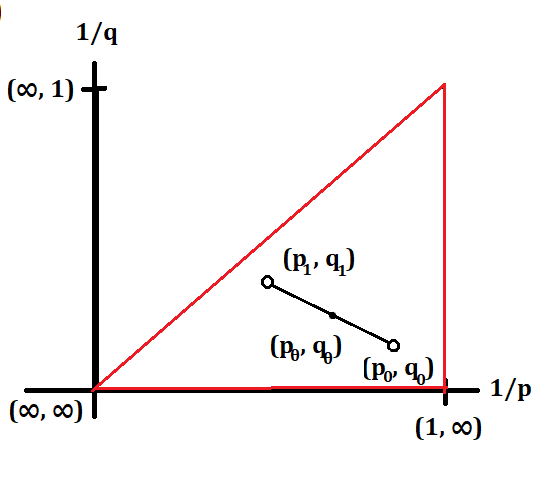
\includegraphics[scale = 0.6]{marcin}
		\caption{The \textit{interpolation diagram}; the restriction $p_0 \leq q_0$ and $p_1 \leq q_1$ guarantees that $p_\theta \leq q_\theta$, so the intermediate line lies on the lower triangle.}
	\end{center}
\end{figure}


\begin{proof}
	Suppose $p_0 < p_1$, then recalling weak-type implies restricted weak-type, we apply Hunt interpolation for $r = q_\theta$ and use the embedding $L^{p_\theta, q_\theta} (X) \subseteq L^{p_\theta, p_\theta} (X)$ which holds since $p_\theta \leq q_\theta$, 
		\[ ||Tf||_{L^{q_\theta}} = ||Tf||_{L^{q_\theta, q_\theta}}^* \lesssim ||f||_{L^{p_\theta, q_\theta}}^* \lesssim ||f||_{L^{p_\theta, p_\theta}}^* = ||f||_{L^{p_\theta}}. \]
	Assume now $p:= p_0 = p_\theta = p_1$, we have that $T$ is weak-type $(p, q_0)$ and $(p, q_1)$, i.e.
	\begin{align*}
		\nu( |T f| > \lambda) 
			&\lesssim \left(\frac{||f||_{L^p}}{\lambda} \right)^{q_0}, \\
		\nu( |T f| > \lambda) 
			&\lesssim \left(\frac{||f||_{L^p}}{\lambda} \right)^{q_1}.
	\end{align*}
	Taking a layered cake decomposition, and assume without loss of generality $q_0 < q_1$, then 
		\begin{align*}
			||Tf||_{L^{q_\theta}}^{q_\theta}
				&\sim \int_0^\infty \lambda^{q_\theta} \nu (|Tf| > \lambda) \frac{d\lambda}{\lambda} \lesssim \int_0^\infty \lambda^{q_\theta} \min \Big\{ \left(\frac{||f||_{L^p}}{\lambda} \right)^{q_0}, \left(\frac{||f||_{L^p}}{\lambda} \right)^{q_1}  \Big\} \frac{d\lambda}{\lambda} \\
				&\lesssim \int_0^{||f||_{L^p}} \lambda^{q_\theta} \left( \frac{||f||_{L^p}}{\lambda} \right)^{q_0}  \frac{d\lambda}{\lambda} + \int_{||f||_{L^p}}^\infty \lambda^{q_\theta} \left( \frac{||f||_{L^p}}{\lambda} \right)^{q_1}  \frac{d\lambda}{\lambda}  \lesssim ||f||_{L^p}^q.
		\end{align*}
	This completes the proof. 	
\end{proof}
\bibliography{biblio}
\bibliographystyle{alpha} 
\end{document}
